\documentclass[a4paper,11pt,twoside]{article}
\usepackage[T1]{fontenc}
\usepackage[utf8]{inputenc}

\usepackage[margin=1in]{geometry}
\usepackage{amsfonts, amsmath, amssymb}
\usepackage{mathtools}

\usepackage{graphicx}

\usepackage{url}
%%  Defines the command \url{} that can be used to typeset url:s
%%  in text

\usepackage[parfill]{parskip}
\usepackage{ragged2e}

\setcounter{tocdepth}{4}
\setcounter{secnumdepth}{4}


\newcommand*{\pd}[2]{\ensuremath{\dfrac{\partial #1}{\partial #2}}}
\newcommand*{\inpd}[2]{\ensuremath{\frac{\partial #1}{\partial #2}}}
\DeclarePairedDelimiter\floor{\lfloor}{\rfloor}

\title{Dense Face Detection with Convolutional Neural Networks}
\title{Derivation of a Convolutional Neural Network Based Dense Face Detector}
\date{}


\begin{document}

\maketitle
\vfill

\begin{flushright}
\today \\*
Nikita Zozoulenko Na15b \\*
nikita.zozoulenko@gmail.com \\*
Katedralskolan Linköping\\*
Supervisor: Rickard Engström \\*
VT 2017 - HT 2018 \\*
\end{flushright}
\newpage

%start abstract
\Large{\textbf{Abstract}}\\\\
Abstract Here......

In this paper the mathematical model behind the standard Artificial Neural Network and the Convolutional Neural Network is derived. A Convolutional Neural Network is then adapted to read handwritten digits and to make a cutting edge face detector, successfully detecting over 50 faces in a crowded scene.
\newpage
%end abstract

\tableofcontents

\section{Introduction}

\subsection{Background}
Artificial neural networks, or more specifically convolutional neural networks, were popularized 2012 when the model was used to win the annual ImageNet Large-Scale Visual Recognition Challenge, beating all current machine learning models. Today they have achieved state of the art results in areas such as self-driving cars, image classification, object localization, automatic image annotation, semantic segmentation of objects in images and natural language processing. 
\cite{cs231n}

An Artificial neural network is a biologically inspired machine learning model that tries to replicate the way the brain in mammals functions. There are many different kinds of Artificial neural networks which vary in structure and architecture. The basic principle behind neural networks is that they are made out of a number of layers of neurons. The layers are built recursively such that the output of one layer is the input of the next layer. They are stacked on top of each other and the number of layers an Artificial neural network has is called its depth. How the neurons of the previous layer are connected to the neurons of the next layer depends on what type on Artificial neural network it is.
\cite{cs231n}

\subsection{Purpose}
When I was first starting out in the field of deep learning I found there was a lack of fully derived explanations of the underlying mathematics behind artificial neural networks. Sources had either only explained one simple forward pass through the network, or had only derived the most simple case, ignoring the more complicated general case. The aim of this paper is to present a clear derivation of the general case for Feed-forward neural networks and Convolutional neural networks. Furthermore, the aim is to apply the derived model of the Convolutional neural network to two problems: Classifying handwritten digits and to detect and pinpoint the location of a variable number of human faces in an image.

\subsection{Problem statement}
What is a Feedforward neural network and Convolutional neural network?
What is forward- and backpropgation and how is it derived in a Feedforward neural network and a Convolutional neural network?
Can an Artificial neural network be trained to classify handwritten digits and detect a variable number of faces in images?

\newpage
\section{Metod}
The majority of the paper and the derivations of the models are based on the course material from Stanford's "CS231n: Convolutional neural networks for Visual Recognition" course. Some advanced concepts were taken from the papers they were introduced in (e.g. Batch Normalization) and expanded to fit the general case of an arbitrary input to the model. The general case for the mathematical model of the Feedforward neural network and the Convolutional neural network were derived by hand and implemented in C++ with the linear algebra library Eigen and in Python in pure NumPy, a library for scientific computing. The derived partial derivatives required by the models were compared with their numerical approximations using the formal definition of a derivative. 

When my own implementation of the Artificial neural networks became too computationally expensive and inefficient for the two problem cases classification of handwritten digits and dense face detection I implemented the models in Google's machine learning library TensorFlow and Facebook's GPU-accelerated tensor and dynamic neural network library PyTorch.

\newpage
\section{Resultat}

\subsection{Feed-forward neural networks}
A feed-forward neural network is the most elementary version of an artificial neural network. As all varying kinds of neural networks, a feed-forward neural network is made out of a number of layers of neurons. The unique property of a feed-forward neural network is that all the neurons in a layer are connected to every neuron in the next layer (see figure \ref{figfeedforward}). \cite{cs231n}

\begin{figure}[h]
	\centering
  		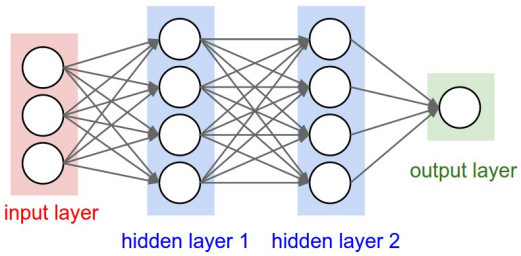
\includegraphics[scale=1]{feedforward.png}
  	\caption{An illustration of a simple feed-forward neural network. It consists of 4 layers: 1 input layer (red), 2 hidden layers (blue) and 1 output layer (green). A circle represents a neuron. Every neuron in a layer is connected to all the neurons in the following layer, shown by the grey lines between the neurons. GLÖM INTE ATT REFERERA} \label{figfeedforward}
\end{figure}

A neuron is represented as a floating point decimal number. The value of a neuron is called its activation. Given an input of $n$ data points the model wants to predict $m$ different values where $n$ and $m$ are the number neurons in the input and output layers. Every data point or feature in the input are set as neurons in the input layer. For instance, if you want to predict a score given 12 different variables every single variable would correspond to one neuron in the input layer of size 12 and the score would correspond to a single neuron in the output layer of size 1. The value of the input neurons are transferred over to the next layer depending on the strength of the different connections every neuron has to the neurons in the next layer. This is repeated for every layer until the signal has reached the output layer. The process of propagating the value of the neurons from the input layer to the output layer is called forward propagation. \cite{cs231n}

The network is trained to predict correct values by optimizing the fixed connections, also called weights, between all the layers in the neural network. \cite{cs231n}

%values by defining a cost function such that the smaller the loss the higher quality the predicted value has.

\subsubsection{Tensors, indexing and notation}
A tensor is the generalization of vectors and matrices. Scalars are tensors of order 0. A tensor of order 1 is a vector $x \in \mathbb{R}^N$ and is a row vector with $N$ elements. It can also be seen as a one-dimensional array. Matrices $M$ are tensors of order 2 such that $M \in \mathbb{R}^{R \times N}$ and can be viewed as a vector of $R$ elements where every element is another vector with $N$ scalar elements. Matrices can also be seen as a two-dimensional array with $RN$ elements. A tensor of order $n$ is an $n$-dimensional array and is indexed by an $n$-tuple. For instance, a tensor $X \in \mathbb{R}^{R \times C \times H \times W}$ is indexed by the four-tuple $(r,c,h,w)$ where $0 \leq r < R$, $0 \leq c < C$, $0 \leq h < H$ och $0 \leq w < W$. \cite{cs231n}

\subsubsection{Forward propagation}
In figure \ref{figfeedforward} only a single training example was worked on at a time. In practice a mini-batch of $R$ training examples are propagated forward in a neural network at the same time. \cite{cs231n} \cite{wikiStanford}

Let $M$ denote the number of layers in the neural network and $l$; $0 \leq l < M$, one specific layer in the neural network. Let $N^{(l)}$ denote the number of neurons in layer $l$. The activation of layer $l$ can be expressed as a tensor of order 2: $X^{(l)} \in \mathbb{R}^{R \times N^{(l)}}$ indexed by the two-tuple $(r,i)$ where $0 \leq r < R$ and $0 \leq i < N$. In addition to the normal neurons a layer has, let $b^{(l)}$ be a bias neuron for the layer $l$ (see figure \ref{figFCCmath}). It is called a bias neuron because its value is independent to what input the neural network is given. \cite{cs231n} \cite{wikiStanford}

The weights expressing how strong the connection between the neurons of layer $l$ and $l+1$ are can also be expressed as a tensor of order 2. Let $W^{(l)} \in \mathbb{R}^{N^{(l+1)}  \times N^{(l)}}$ such that the element $W_{j, i}^{(l)}$ is the strength of the connection between neuron $X_{ri}^{(l)}$ and $X_{rj}^{(l+1)}$ for arbitrary example $r$ in the mini-batch. \cite{cs231n} \cite{wikiStanford}

\begin{figure}[h]
	\centering
  		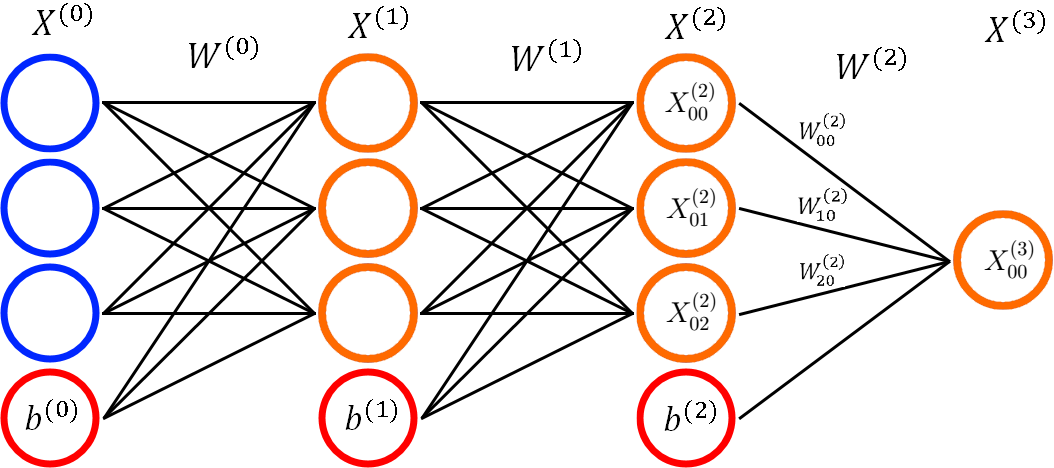
\includegraphics[scale=0.4]{FCC.png}
  	\caption{An example of a 4 layer feed-forward neural network. The input neurons are marked with blue. The bias neurons are marked with red. Black lines between neurons symbolyze the weights between every pair of neurons between two layers.} \label{figFCCmath}
\end{figure}

To calculate the value of a neuron in layer $l+1$ every neuron in layer $l$ is multiplied by its corresponding weight in $W^{(l)}$ and summed together with the layers bias neuron. The sum is then put in a so called activation function $f$. The value of the activation function is the neurons activation in layer $l+1$. \cite{cs231n} \cite{wikiStanford}

Let $Z^{(l)} \in \mathbb{R}^{R \times N^{(l)}}$ be the value of each neuron in layer $l$ before being put into the activation function. Given an input $X^{(0)}$ the forward propagation can be expressed recursively as: \cite{cs231n} \cite{wikiStanford}

\begin{align}
Z_{rj}^{(l+1)} & = b^{(l)} + \sum^{N^{(l)}-1}_{i = 0} X^{(l)}_{r,i} W^{(l)}_{i,j}\\
X_{rj}^{(l+1)} & = f(Z_{rj}^{(l+1)})
\end{align}

The tensor of activations and weights are constructed in such as way that one forward pass through a single layer can be computed with a single dot product and having the bias term added to every element in the computed dot product. The activation function $f$ is then applied element-wise on each neuron: \cite{cs231n} \cite{wikiStanford}

\begin{align}
Z^{(l+1)} & = X^{(l)}W^{(l)}+b^{l}\\
X^{(l+1)} & = f(Z^{(l+1)})
\end{align}

Common activation functions are Rectified Linear Units (ReLU), sigmoid ($\sigma$) and hyperbolic tangent ($\tanh$) and are defined by equation \eqref{relu} - \eqref{tanh} (see figure \ref{activation_function}). A non-linear activation function is chosen to enable the network to make use of non-linearities when learning to predict values. Without non-linear activation functions the whole model is equivalent to one large linear transformation of the input data. \cite{cs231n}

\begin{equation}\label{relu}
\mbox{ReLU}{(x)} = \begin{cases} 
			0 & \mbox{if } x < 0 \\ 
			x & \mbox{if } x \geq 0 
		\end{cases}
\end{equation}

\begin{equation}\label{sigmoid}
\sigma(x) = \frac{1}{1+e^{-x}}
\end{equation}

\begin{equation}\label{tanh}
\tanh{(x)} = \frac{e^x-e^{-x}}{e^x+e^{-x}}
\end{equation}

\begin{figure}[h]
	\centering
  		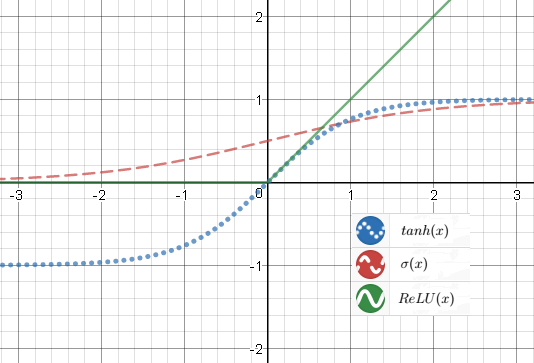
\includegraphics[scale=0.83]{activationfunction.png}
  	\caption{A graph of ReLU, $\sigma$ och $\tanh$.} \label{activation_function}
\end{figure}

\subsubsection{Cost function}
Given an input $X$ and a ground truth $y$ the model wants to predict values $\hat{y}$ which resembles the ground truth as closely as possible. It is achieved by defining a multivariate cost function $L(\theta; X, y)$  with the network's parameters $\theta$ (all the weights and biases) with respect to a single training example $(X, y)$. The cost function describes the quality of the prediction $\hat{y}$ such that a lower cost represents a more accurate prediction. One way of defining the cost function is to use the mean squared error as in equation \eqref{MSE}:

\begin{equation}\label{MSE}
L(\theta) = \frac{1}{RN} \sum^{R-1}_{r=0} \sum^{N-1}_{i=0} (\hat{y}_{r,i}-y_{r,i})^2
\end{equation}
%& = {||f(f(f(XW^{(0)} +b^{(0)})W^{(1)} +b^{(1)})W^{(2)} +b^{(2)}) - y||}^2
Where $R$ is the batch size and $N$ is the number of features in the last layer.

The neural network is trained to predict accurate results by iterating through the training data and minimizing the cost function. Since the given input $X$ stays fixed, the network learns to optimize its weights $W^{(l)}$ and biases $b^{(l)}$ for every layer $l$.

\subsubsection{Gradient Descent}
The gradient $\nabla L(\theta)$ is a vector of partial derivatives with respect to the parameters $\theta$ of the function $L$ defined by equation \eqref{EQgradient} and \eqref{EQgradientvector}: \cite{gradient} \cite{convmath} 
\begin{equation}\label{EQgradient}
\nabla L(\theta) : \mathbb{R}^n \to \mathbb{R}^n
\end{equation}
\begin{equation}\label{EQgradientvector}
\nabla L(\theta) = 
	\begin{pmatrix} 
		\pd{L(\theta)}{\theta_{0}}, & 
		\pd{L(\theta)}{\theta_{1}}, &
		\cdots, &
		\pd{L(\theta)}{\theta_{n-1}}
		
		\end{pmatrix}
\end{equation}

The gradient $\nabla L(\theta)$ shows the direction of steepest ascent in the point ($\theta_{0}$, $\theta_{0}$, ..., $\theta_{0}$) in the $n$-dimensional vector space $\mathbb{R}^{n}$. For a function $f(x)$ of a single variable $x$, the gradient is simply the derivative of the function with respect to $x$ and is the slope of the tangent line to $f$ at $x$. For a multivariate function $f(x,y)$ of two variables $x$ and $y$ the gradient would be the a two-dimensional vector of the slope in the x dimension and y dimension respectively. 

Gradient descent is the method of iteratively changing the values of $\theta$ proportionally to the negative gradient $-\nabla L(\theta)$ to minimize the function $L(\theta)$ (see figure \ref{figSGD}). The most basic version of gradient descent is called Stochastic Gradient Descent (SGD) and uses the hyperparameter $\alpha$, called learning rate, to control the magnitude of the gradient. Stochastic Gradient Descent is defined by equations (\ref{EQgradient}) and (\ref{SGD}).

\begin{equation}\label{EQgradient}
\pd{L(\theta)}{\theta^{(l)}} = \nabla_{\theta^{(l)}} L(\theta)
\end{equation}
\begin{equation}\label{SGD}
\theta^{(l)} \to \theta^{(l)} - \alpha \pd{L(\theta)}{\theta^{(l)}}
\end{equation}
\begin{figure}[h]
	\centering
  		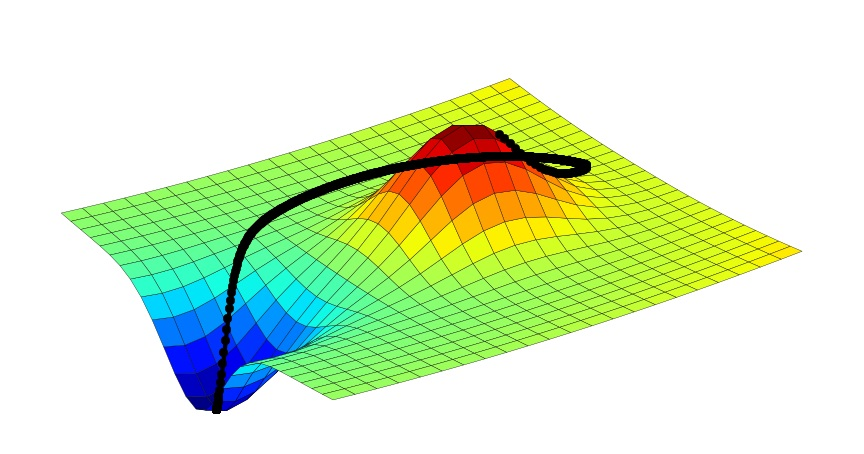
\includegraphics[scale=0.5]{SGD.png}
  	\caption{An illustration of Stochastic Gradient Descent on a function of two variables. Red symbolizes a high value of the function while blue symbolizes a low value. The parameters are initialized at the global maximum and their values are altered iteratively to move in the direction of the negative gradient: the direction of steepest descent. \cite{figSGD}} \label{figSGD}
\end{figure}

\subsubsection{Backpropagation}
Nätverket tränas genom att varje träningsexempel $(X,y)$ framåtpropageras och insätts i kostnadsfunktionen $L$. Genom processen som kallas för bakåtpropagering beräknas alla partiella derivator med avseende på en viss vikt och används för att uppdatera vikterna tills nätverkets prognos liknar de sanna värdena. \cite{gradient} \cite{convmath} \cite{wikiStanford}

Backpropagation stands for "backwards propagation of errors" and is the process of calculating the partial derivatives of the loss function with respect to the model's parameters, or in other terms calculating the gradient. \cite{wikiStanford} \cite{gradient}

The partial derivatives can be approximated numerically with the formal definition of a derivative defined by equation (\ref{EQderivativeDefinition}): \cite{wikiStanford} \cite{gradient}

\begin{equation}\label{EQderivativeDefinition}
\pd{L(\theta)}{\theta_{i}} = \frac{L(\theta_{0},...,\theta_{i} + h, ..., \theta_{n-1})-L(\theta)}{h}
\end{equation}

This would not be a problem for the small neural network in figure \ref{figFCCmath} with a total of 24 parameters, but would be extremely inefficient for deep neural networks with millions of parameters. Instead, the chain rule is applied to calculate the precise value of the partial derivatives.

Let $\delta^{(l)}$ denote the so called delta error at layer $l$, defined by equation (\ref{deltaerrordefinition}):

\begin{equation}\label{deltaerrordefinition}
\inpd{L(\theta)}{X^{(l)}} = \delta^{(l)}
\end{equation}

The delta error is the partial derivative of the loss with respect to a specific neuron in model and is needed to efficiently calculate the gradient. The delta error can be interpreted as how much a specific neuron affects the total loss of the cost function. A deviation in value of a neuron with a big delta error results in a greater change of the total loss compared to a neuron with a small delta error. Because the activation of layer $l+1$ is a function of the previous layer $l$, the delta error can be computed recursively from the output layer and propagated backwards to the first layer in the network. By applying the chain rule the delta error $\inpd{L(\theta)}{X^{(l)}}$  at layer $l$ can be broken up into three partial derivatives $\inpd{L(\theta)}{X^{(l+1)}_{r,j}}$, $\inpd{X^{(l+1)}_{r,j}}{Z^{(l+1)}_{r,j}}$ and $\inpd{Z^{(l+1)}_{r,j}}{X^{(l)}_{r,i}}$. Since a single neuron in layer $l$ is connected to every neuron in layer $l+1$ you have to sum over every neuron in layer $l+1$. The first partial derivative is the delta error of the next layer and the other two partial derivatives can be derived from equations (1) and (2) and are easily differentiable since they are linear equations:
\begin{equation}\label{dLdX_FCC}
\begin{split}
\delta^{(l)}_{r,i}
	& = \pd{L(\theta)}{X^{(l)}_{r,i}}  \\
	& = \sum^{N^{(l+1)}}_{j=0} \pd{L(\theta)}{X^{(l+1)}_{r,j}} \pd{X^{(l+1)}_{r,j}}{Z^{(l+1)}_{r,j}} \pd{Z^{(l+1)}_{r,j}}{X^{(l)}_{r,i}} \\
	& = \sum^{N^{(l+1)}}_{j=0} \delta^{(l+1)}_{r,j} f'(Z^{(l+1)}_{r,i}) \ W^{(l)}_{j,i} 
\end{split}
\end{equation}

The delta error of the last layer $L-1$ depends on what loss function is used. For the mean squared error the delta error of the output layer is defined by equation (\ref{MSEdelta}): 

\begin{equation}\label{MSEdelta}
\begin{split}
\delta^{(l_{sista})}
	& = \pd{L(\theta)}{\hat{y}}  \\
	& = \frac{2}{RN} (\hat{y}-y)
\end{split}
\end{equation}

With the delta error defined at every layer in the network the partial derivative of the loss function with respect to the networks parameters can be calculated. Just like equation (\ref{dLdX_FCC}) $\inpd{L(\theta)}{X^{(l)}}$ is broken up into three partial derivatives $\inpd{L(\theta)}{X^{(l+1)}_{r,i}}$, $\inpd{X^{(l+1)}_{r,i}}{Z^{(l+1)}_{r,i}}$ and $\inpd{Z^{(l+1)}_{r,i}}{W^{(l)}_{i,j}}$. All the examples in the mini-batch are summed over since the weights affect every single example. $\inpd{L(\theta)}{X^{(l+1)}_{r,i}}$ is the delta error and the other two partial derivatives are derived from equations (1) and (2):

\begin{equation}\label{dLdW_FCC}
\begin{split}
\pd{L(\theta)}{W^{(l)}_{j,i}} 
	& = \sum^{R-1}_{r=0} \pd{L(\theta)}{X^{(l+1)}_{r,i}} \pd{X^{(l+1)}_{r,i}}{Z^{(l+1)}_{r,i}} \pd{Z^{(l+1)}_{r,i}}{W^{(l)}_{i,j}} \\
	& = \sum^{R-1}_{r=0} \delta^{(l+1)}_{r,i} f'(Z^{(l+1)}_{r,i}) \ X^{(l)}_{r,j}\\
\end{split}
\end{equation}

The partial derivative of the loss function with respect to the biases are found in a similar way to equation (\ref{dLdX_FCC}) and (\ref{dLdW_FCC}):
\begin{equation}\label{dLdb_FCC}
\begin{split}
\pd{L(\theta)}{b^{(l)}} 
	& = \sum^{R-1}_{r=0} \pd{L(\theta)}{X^{(l+1)}_{r,i}} \pd{X^{(l+1)}_{r,i}}{Z^{(l+1)}_{r,i}} \pd{Z^{(l+1)}_{r,i}}{b^{(l)}_{i,j}} \\
	& = \sum^{R-1}_{r=0} \delta^{(l+1)}_{r,i} f'(Z^{(l+1)}_{r,i}) \\
\end{split}
\end{equation}


\subsubsection{Training neural networks}
The model is tra
Bakåtpropageringen sker lager till lager med start i outputlagret. Vid varje lager måste delta-felet $\delta^{(l)}$ bakåtpropageras och derivatan av det lagrets parametrar $W^{(l)}$ och $b^{(l)}$ beräknas. \cite{cs231n}

Neurala nätverk tränas genom att iterativt uppdatera nätverkets vikter med hjälp av \textit{gradient descent}. Den hela träningsdatabasen delas in i mini-hopar och väljs ut slumpvist. En iteration av SGD appliceras genom att framåtpropagera ett träningsexempel och sedan bakåtpropagera felet för att beräkna gradienten av kostnadsfunktionen med avseende på alla vikter i närverket. Denna process upprepas tills nätverkets vikter konvergerar och nätverkets prognos efterliknar verkligheten. \cite{cs231n}

Två implementationer av ett feed-forward neuralt nätverk kan hittas på github i python och C++: \url{https://github.com/nikitazozoulenko}

\subsection{Konvolutionella neuala nätverk}
När människor vill identifiera någonting i en bild så letar vi efter vissa karakteristiska drag objektet har. En hund består exempelvis av en kropp, ett huvud och fyra ben. Kroppsdelarna består sedan själva av grundläggande geometriska former som i sig självt är kombinationer av kanter och linjer. Dessutom har hundar en viss textur, det som vi kännetecknar som något pälsliknande. Dessa karakteristiska drag är lokala inom bilden och kan extraheras av att endast se på en liten del av bilden i taget. Detta är principen bakom \textit{Konvolutionella Neurala Nätverk (CNN)}: Genom så kallade \textit{konvolutioner} kunna extrahera dessa karakteristiska drag. Nätverket lär sig ett antal små filter som den applicerar på en delmängd av bilden genom att filtret sammanrullar över hela bilden (se figur 4). Värdet av filtret över en delmängd av bilden blir aktiveringen av ett neuron i nästa lager. \cite{cs231n}

\begin{figure}[h]\label{figkatter}
	\centering
  		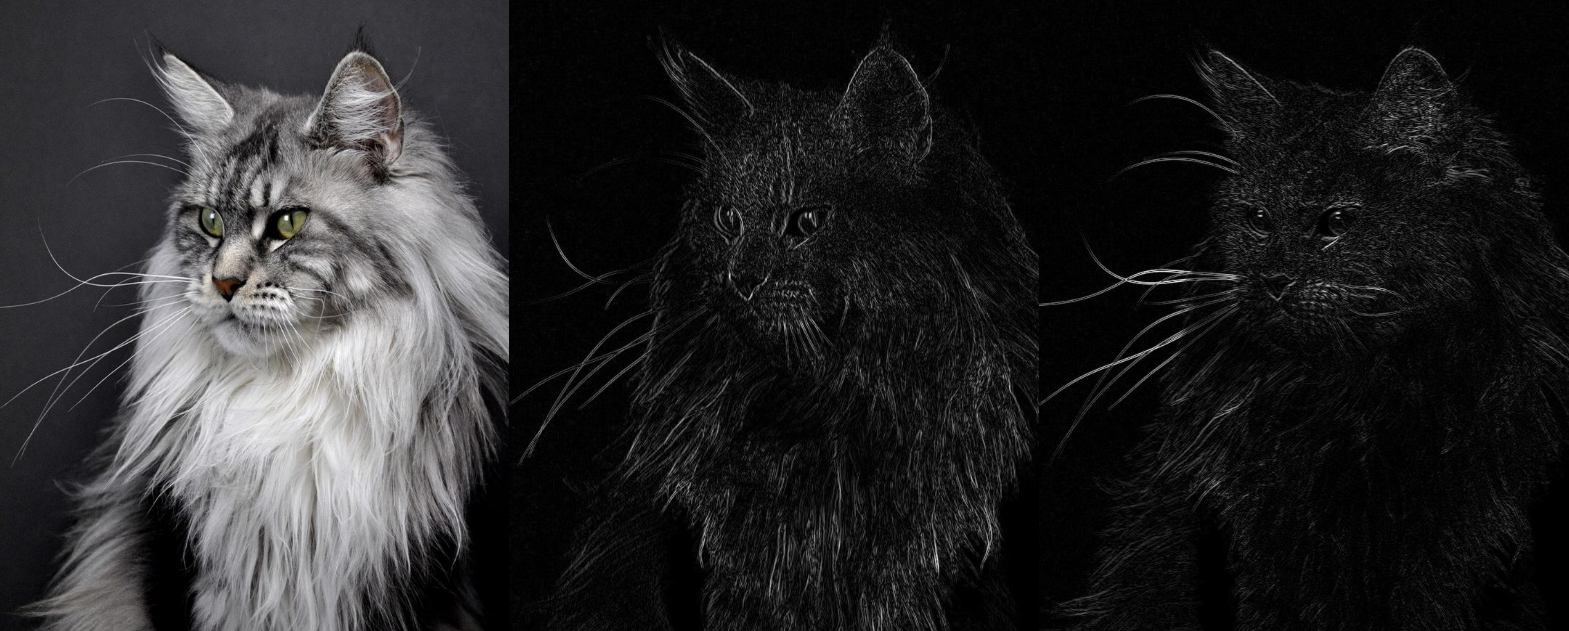
\includegraphics[scale=0.33]{katter.png}
  	\caption{Resultatet av att ett filter för vertikal respektive horizontell kantdetektering har sammanrullat över en bild av en katt.}
\end{figure}

Till skillnad från \textit{FCC} är neuronerna i ett \textit{CNN} bara kopplade till närliggande neuroner i det föregående lagret. På detta sätt kan nätverket lära sig fler hög-nivåspecialartiklar ju djupare i nätverket signalen går. Exempelvis kan det hända att det första lagret lär sig att identifiera kanter och linjer medan de senare lagren lagren lär sig att känna igen olika geometriska former och till sist känna igen ansikten eller object i det sista lagret. \cite{cs231n}

Modellen, precis som ett \textit{feed-forward nätverket}, består av ett flertal lager neuroner sådant att resultatet av ett lager matas in till nästkommande lager. Det sista lagret benämns med $X^{(l_{sista})}$ eller $\hat{y}$. Vid varje lager finns dessutom vikter $W^{(l)}$  som beror på vad för slags lager det är. $W^{(l)}$ kan vara tom med inga vikter när lager inte bidrar till någon inlärning. Ekvation \eqref{CNNeq} illustrerar strukturen av modellen.\cite{cs231n} \cite{convmath}
\begin{equation}\label{CNNeq}
X^{(0)} \xrightarrow{W^{(l)}} X^{(1)}  \xrightarrow{W^{(l)}} \cdots  \xrightarrow{W^{(l_{sista}-2)}} X^{(l_{sista}-1)}  \xrightarrow{W^{(l_{sista}-1)}} X^{(l_{sista})} = \hat{y}
\end{equation}

Samtliga olika typer av lager i en konvolutionellt neuralt nätverk har två olika faser: framåtpropagering och bakåtpropagering. Vid framåtpropagering används aktiveringen av det föregående lagret för att beräkna aktiveringen vid nästintilliggande lager. Vid bakåtpropagering måste det rekursiva delta-felet propageras baklänges i nätverket med hjälp av kedjeregeln för att sedan beräkna den paritella derivatan av lagrets vikter med avseende på kostnadsfunktionen. \cite{cs231n}

För ett feed-forward neuralt nätverk används matriser för att representera neuronerna. I ett \textit{CNN} är en tensor $X^{(l)} \in \mathbb{R}^{R \times C  \times H \times W}$ med ordning 4 aktiveringen vid lager $l$ och indexeras med fyr-tupeln $(r,c,h,w)$ där $0 \leq r < R$, $0 \leq c < C$, $0 \leq h < H$ och $0 \leq w < W$. Aktiveringarna vid nästintilliggande lager $l+1$ betecknas med $X^{(l+1)} \in \mathbb{R}^{R \times C' \times H' \times W'}$ och indexeras med fyr-tupeln $(r,c',h',w')$ där $0 \leq r < R$, $0 \leq c' < C'$, $0 \leq h' < H'$ och $0 \leq w' < W'$. \cite{cs231n} \cite{convmath}








Aktiveringen brukar illustreras som en tredimensionell volym där $W$, $H$ och $C$ är bredden, höjden respektive djupet. En $H \times W$ skiva av volymen kallas för en \textit{feature map} eller en \textit{kanal}. Antalet kanaler betecknas med $C$. $R$ står för hopstorlek då man bearbetar R exempel i taget i en så kallad mini-hop. \cite{cs231n} \cite{convmath}

\begin{figure}[h]\label{figboatcnn}
	\centering
  		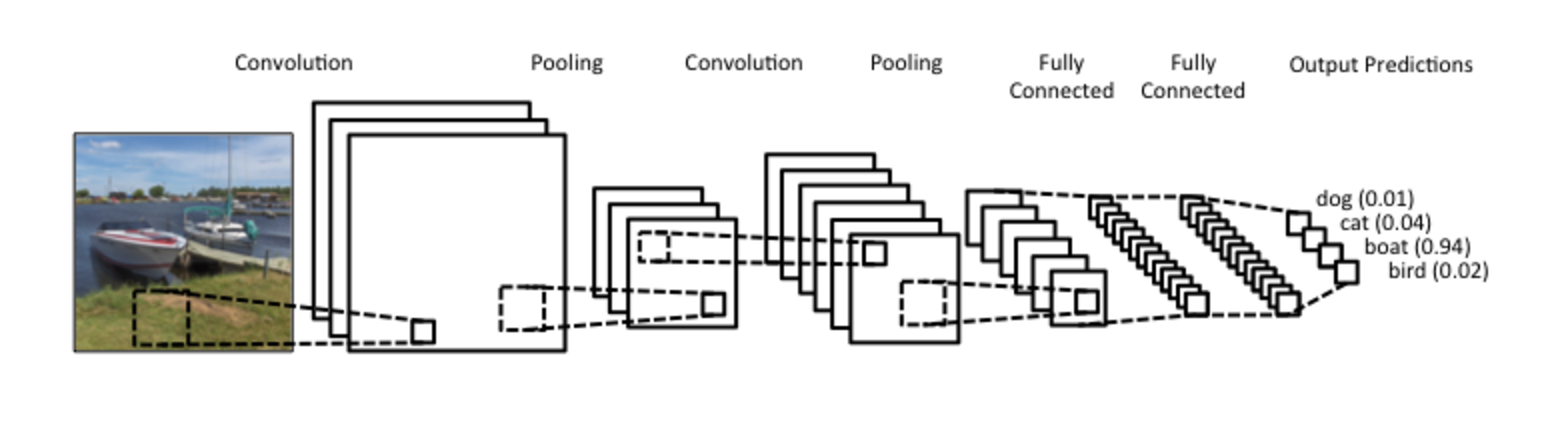
\includegraphics[scale=0.6]{boatcnn.png}
  	\caption{En illustration av ett konvolutionellt neuralt nätverk. Varje skiva är en egen \textit{feature map}. \cite{figboatcnn}}
\end{figure}

På grund av att en konvolution är en lokal operator används CNN:s för data som innehåller lokalt sammanhängande samband, exempelvis bilder eller ljud. Om det är en bild som bearbetas har det första lagrets aktivering $C = 3$ kanaler, en för varje RGB-kanal, och en bredd och höjd lika med bildens bredd och höjd i pixlar. \cite{cs231n} \cite{convmath}

\subsubsection{Konvolutionslagret framåtpropagering}
Ett konvolutionslager består av ett antal vikter kallade \textit{kärnor (kernels)} eller \textit{masker (masks)}, representerade av en tensor med ordning fyra, $W^{(l)} \in \mathbb{R}^{C' \times C  \times K_h \times K_W}$ för lager $l$. \cite{cs231n} \cite{convmath}

När masken är över en godtycklig del av volymen multipliceras varje värde i delmängden av $W^{(l)}$ elementvis med respektive värde i masken vid samma position och summeras (se figur 6). Summan blir aktiveringen av ett neuron i nästa lager. Konvolutionsoperatorn betecknas med $*$. \cite{cs231n} \cite{convmath}

\begin{figure}[h]\label{figkonv}
	\centering
  		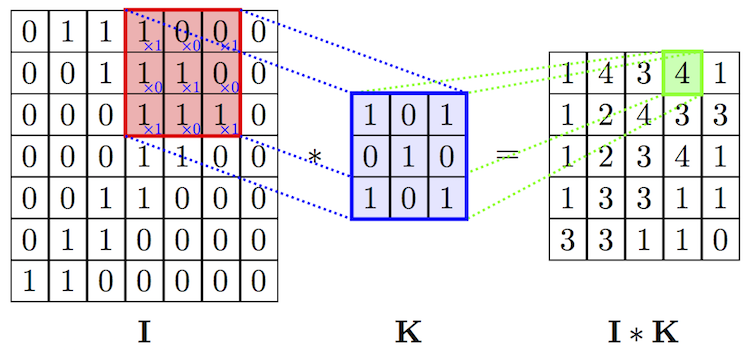
\includegraphics[scale=2.1]{convolution.png}
  	\caption{En kärna med storlek $3 \times 3$ sammanrullar över ett område med dimensioner $6 \times 6$ och bildar en aktivering med dimensionerna $4 \times 4$. \cite{figkonv}}
\end{figure}

En feature map i lager $l+1$ är resultatet av att en kärna med dimensioner $1 \times \times C  \times K_h \times K_W$ har sammanrullat över aktiveringen av det föregående lagret. $C'$ är antalet kärnor och blir dessutom antalet feature maps nästa lager har. \cite{cs231n} \cite{convmath}

Kärnorna har två ytterligare egenskaper: ett kliv $s$ och så kallad \textit{zero-padding} $p$. $s$ är hur stort kliv man tar efter varje gång filtret blir applicerat på tensorn. Man ökar tensorns höjd och bredd med $2p$ genom att fylla på med nollor vid tensors ändor (se figur 7). På grund av att aktiveringens höjd och bredd avtar ju djupare i nätverket de befinner sig på används zero-padding för att kontrollera storleken av tensorn. \cite{cs231n} \cite{convmath} \cite{convarithmetic}

\begin{figure}[h]\label{figzeropad}
	\centering
  		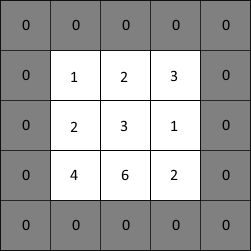
\includegraphics[scale=0.7]{zeropadding.png}
  	\caption{Ett område med dimensioner $3 \times 3$ zero-paddas med $p=1$ och resulterande område får dimensioner $5 \times 5$.}
\end{figure}

Låt $W^{(l)} \in \mathbb{R}^{C' \times C  \times K_h \times K_W}$, $X^{(l)} \in \mathbb{R}^{R \times C  \times (H+2p) \times (W+2p)}$ och $X^{(l+1)} \in \mathbb{R}^{R \times C'  \times H' \times W'}$. Dimensionerna vid lager $l+1$ beskrivs av: \cite{cs231n} \cite{convmath} \cite{convarithmetic}
\begin{equation}
W' = \frac{W-K_W+2p}{s} +1
\end{equation}
\begin{equation}
H' = \frac{H-K_H+2p}{s} +1
\end{equation}

Då beskrivs en konvolution algebraiskt genom: \cite{cs231n} \cite{convmath}
\begin{equation}
w = sw'
\end{equation}
\begin{equation}
h = sh'
\end{equation}
\begin{equation}\label{konvolution}
\begin{split}
	\begin{bmatrix} X^{(l+1)} \end{bmatrix}_{r, c', h', w'}	
		& = X^{(l)}_{r, c', h', w'} *W^{(l)}_{c'} \\
		& = \sum^{C-1}_{c=0} \sum^{K_H-1}_{j=0} \sum^{K_W-1}_{i=0} X^{(l)}_{r, c, h'+j, w'+i}W^{(l)}_{c', c, j, i}
\end{split}
\end{equation}

Index på termen som ska sammanrullas i konvolutionen symboliserar vilka dimensioner som ska summeras. Exempelvis visar $W^{(l)}_{c'}$ att dimensionerna $C$, $H$ och $W$ (alla kanaler) ska summeras medan  $W^{(l)}_{c', c}$ visar att endast $H$ och $W$ (en kanal) ska summeras.

I praktiken brukar konvolutioner implementeras med hjälp av funktionerna $row2im$ och $im2row$ vilka möjliggör att en konvolution att beräknas med en matrismultiplikation. \cite{cs231n} \cite{convmath} \cite{convarithmetic}

\subsubsection{Konvolutionslagret bakåtpropagering}
Vid varje lager $l$ bakåtpropageras det rekursiva delta-felet $\delta$ och den partiella derivatan av lagerts vikter med avseende på kostnadsfunktionen $L$ beräknas. 

Bakåtpropageringen av det rekursiva delta-felet $\inpd{L(W)}{X^{(l+1)}_{r,c',h',w'}}$ räkas ut med hjälp av kedjeregeln. Derivatan kan inte endast delas upp i $\inpd{L(W)}{X^{(l+1)}_{r,c',h',w'}}$ och $\inpd{X^{(l+1)}_{r,c',h',w'}}{X^{(l)}_{r,c,h,w}}$, utan alla derivator måste summeras på grund av att det är mer än ett neuron som är ansvarig för framåtpropageringen likt ekvationer \eqref{dLdW_FCC}, \eqref{dLdb_FCC} och \eqref{dLdX_FCC}. $X^{(l+1)}_{r,c',h',w'}$ byts sedan ut mot dess definition enligt ekvation \eqref{konvolution}. \cite{convmath} \cite{webconv1} \cite{webconv2} \cite{webconv3}
\begin{equation}\label{konvolutionbackprop}
\begin{split}
	\delta^{(l)}_{r,c,h,w}
		& = \pd{L(W)}{X^{(l)}_{r,c,h,w}} \\
		& = \sum^{C'-1}_{c'=0} \sum^{H'-1}_{h'=0} \sum^{W'-1}_{w'=0} \pd{L(W)}{X^{(l+1)}_{r,c',h',w'}} \pd{X^{(l+1)}_{r,c',h',w'}}{X^{(l)}_{r,c,h,w}} \\
		& = \sum^{C'-1}_{c'=0} \sum^{H'-1}_{h'=0} \sum^{W'-1}_{w'=0} \delta^{(l+1)}_{r,c',h',w'} \pd{\sum^{C-1}_{c=0} \sum^{k_H-1}_{j=0} \sum^{k_W-1}_{i=0} X^{(l)}_{r, c, h'+j, w'+i}W^{(l+1)}_{c', c, j, i}}{X^{(l)}_{r,c,h,w}}
\end{split}
\end{equation}

Varje produkt i den innersta summan kommer att vara lika med noll förutom om $X^{(l)}_{r, c, h'+j, w'+i} = X^{(l)}_{r,c,h,w}$. Förljaktligen insätter man $h'+j = h$ och $h'+j = h$. Summorna och derivatan förkortas: \cite{webconv1} \cite{webconv2} \cite{webconv3}
\begin{multline}
\sum^{C'-1}_{c'} \sum^{H'-1}_{h'=0} \sum^{W'-1}_{w'=0} \delta^{(l+1)}_{r,c',h',w'} \pd{\sum^{C-1}_{c=0} \sum^{K_H-1}_{j=0} \sum^{K_W-1}_{i=0} X^{(l)}_{r, c, h'+j, w'+i}W^{(l+1)}_{c', c, j, i}}{X^{(l)}_{r,c,h,w}} \\
	 = \sum^{C'-1}_{c'=0} \sum^{H'-1}_{h'=0} \sum^{W'-1}_{w'=0} \delta^{(l+1)}_{r,c',h',w'} W^{(l+1)}_{c', c, j, i} \\
	 = \sum^{C'-1}_{c'=0} \sum^{H'-1}_{h'=0} \sum^{W'-1}_{w'=0} W^{(l+1)}_{c', c, (h-h'), (w-w')}  \delta^{(l+1)}_{r,c',h',w'}   \\
\end{multline}
Vilket man kan se är en summa av konvolutioner där en viss \textit{feature map} av delta-felet sammanrullar över alla kärnor på en viss \textit{feature map} med vikter som är roterade $180^\circ$. För att en konvolution ska kunna ske måste den roterade vikten zero-paddas på grund av att det glidande fönstret måste vara som mest lika stor som tensorn den sammanrullar över. Låt rotationen betecknas med funktionen $rot()$. \cite{webconv1} \cite{webconv2} \cite{webconv3}
\begin{equation}
\delta^{(l)}_{r,c,h,w} = \sum^{C'-1}_{c'=0} rot(W^{(l+1)}_{c',c,h,w}) * \delta^{(l+1)}_{r,c'}
\end{equation}
En sundshetskontroll visar att detta är intuitivt då alla \textit{feature maps} i $X^{(l)}$ används för att skapa en enstaka \textit{feature map} i $X^{(l+1)}$. Det är därför man summerar över alla kärnor och endast konvolverar i en \textit{feature map} i taget och summerar alltihop. \cite{cs231n}

Den partiella derivatan av kostandsfunktionen med avseende på vikterna hittas på ett liknande sätt. Här summeras dessutom $R$-dimensionen på grund av att alla exempel i mini-hopen har en påverkan på gradienten: \cite{cs231n} \cite{webconv1} \cite{webconv2} \cite{webconv3} 
\begin{align}
\begin{split}
	\pd{L(W)}{W^{(l)}_{c',c,h,w}}
		& = \sum^{R-1}_{r=0} \sum^{C'-1}_{c'=0} \sum^{H'-1}_{h'=0} \sum^{W'-1}_{w'=0} \pd{L(W)}{X^{(l+1)}_{r,c',h',w'}} \pd{X^{(l+1)}_{r,c',h',w'}}{W^{(l)}_{r,c,h,w}} \\
		& = \sum^{R-1}_{r=0} \sum_{c'=0}^{C'-1} \sum^{H'-1}_{h'=0} \sum^{W'-1}_{w'=0} \delta^{(l+1)}_{r,c',h',w'} \pd{\sum\limits^{C-1}_{c=0} \sum\limits^{K_H-1}_{j=0} \sum\limits^{K_W-1}_{i=0} X^{(l)}_{r, c, h'+j, w'+i}W^{(l)}_{c', c, j, i}}{W^{(l)}_{c',c,h,w}} \\
		& = \sum^{R-1}_{r=0} \sum^{C'-1}_{c'=0} \sum^{H'-1}_{h'=0} \sum^{W'-1}_{w'=0} X^{(l)}_{r, c, h'+h, w'+w} \delta^{(l+1)}_{r,c',h',w'} \\
		& = \sum^{R-1}_{r=0} \sum^{C'-1}_{c'=0} X^{(l)}_{r, c, h, w} * \delta^{(l+1)}_{r,c'} \\
\end{split}
\end{align}

\subsubsection{Aktiveringsfunktionslager framåtpropagering}
Aktiveringsfunktionen $f$ appliceras elementvis på alla neuroner i $X^{(l)}$. Följaktligen har $X^{(l)}$ och $X^{(l+1)}$ samma dimensioner. Låt aktiveringsfunktionen betecknas med $f$. Nervsignalen framåtpropageras genom: \cite{convmath}
\begin{equation}
X^{(l+1)}_{r,c,h,w} = f(X^{(l)}_{r,c,h,w})
\end{equation}
Aktiveringsfunktioner ökar nätverks precision och får dem att konvergera snabbare, vilket leder till att mindre datakraft krävs för att träna nätverket. \cite{cs231n}

\subsubsection{Aktiveringsfunktionslager bakåtpropagering}
Aktiveringsfunktioner har inga parametrar som ska optimeras och sålades är $W^{(l)}$ och $\inpd{L(W)}{W^{(l)}}$ tomma. Bakåtpropageringen av det rekursiva delta-felet härleds med hjälp av kedjeregeln: \cite{cs231n} \cite{convmath}

\begin{equation}
\begin{split}
\delta^{(l)}_{r,c,h,w}
		& = \pd{L(W)}{X^{(l)}_{r,c,h,w}} \\
		& = \pd{L(W)}{X^{(l+1)}_{r,c,h,w}} \pd{X^{(l+1)}_{r,c,h,w}}{X^{(l)}_{r,c,h,w}} \\
		& = \delta^{(l+1)}_{r,c,h,w} f'(X^{(l)}_{r,c,h,w})
\end{split}
\end{equation}

\subsubsection{Maxpoollagret framåtpropagation}
Här är igen inputneuronerna representerade av $X^{(l)} \in \mathbb{R}^{R \times C \times H \times W}$ och skapar output $X^{(l+1)} \in \mathbb{R}^{R \times C' \times H' \times W'}$. Lagret saknar vikter men har däremot hyperparametrarna $k$ (kärnstorlek) och $s$ (stride eller kliv). \textit{Maxpooling} delar in varje \textit{feature map} i $X^{(l)}$ i ett antal sektioner med dimensioner $k \times k$ genom att ett glidande fönster med samma dimensioner samanrullar över alla lagrets \textit{feature maps} (se figur 8). Aktiveringen vid ett neuron i lager $l+1$ blir lika med det största värdet i korresponderande $k \times k$ sektion. \cite{cs231n} \cite{convmath} \cite{convarithmetic}

\begin{figure}[h]\label{figmaxpool}
	\centering
  		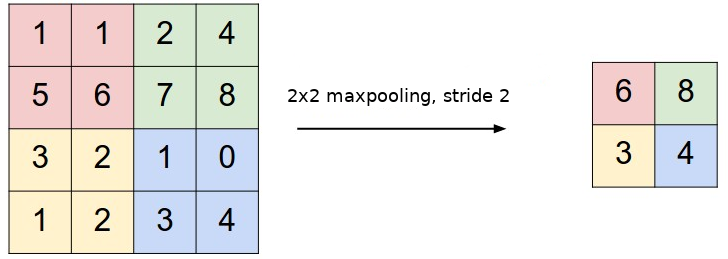
\includegraphics[scale=0.7]{maxpool.png}
  	\caption{Maxpooling med $k=2$ och $s=2$ av ett område med dimensioner $4 \times 4$ där resultatet bildar ett område med dimensionerna $2 \times 2$.}
\end{figure}

Liknande konvolutionslagret utan zero-padding blir det nästintillkommande lagrets dimensioner: \cite{cs231n} \cite{convmath} \cite{convarithmetic}
\begin{equation}
W' = \frac{W-k}{s}+1
\end{equation}
\begin{equation}
H' = \frac{H-k}{s}+1
\end{equation}
\begin{equation}
C' = C
\end{equation}
Antal kanaler förblir konstant. \cite{cs231n} \cite{convmath}

Matematiskt beskrivs maxpoollagret genom: \cite{cs231n} \cite{convmath}
\begin{equation}\label{maxpool}
X^{(l+1)}_{r,c',h',w'} = \underset{0 \leq j < k, \ 0 \leq i < k}{\max} X^{(l)}_{r,c',(h's+j),(w's+i)}
\end{equation}
\subsubsection{Maxpoollagret bakåtpropagering}
Maxpooling saknar vikter och därmed är $\inpd{L(W)}{W^{(l)}}$ tom. Det som återstår är bakåtpropageringen av delta-felet. Med hjälp av kedjeregeln kan man dela upp derivatan i två bråk, $\inpd{L(W)}{X^{(l+1)}_{r,c',h',w'}}$ och $\inpd{X^{(l+1)}_{r,c',h',w'}}{X^{(l)}_{r,c,h,w}}$. $\inpd{L(W)}{X^{(l+1)}_{r,c',h',w'}}$ är den rekursiva delta-delet. $X^{(l+1)}_{r,c',h',w'}$ byts sedan ut mot dess definition enligt ekvation \eqref{maxpool}: \cite{cs231n} \cite{convmath} \cite{webconv3}

\begin{equation}
\begin{split}
	\delta^{(l)}_{r,c,h,w}
		& = \pd{L(W)}{X^{(l)}_{r,c,h,w}} \\
		& = \pd{L(W)}{X^{(l+1)}_{r,c',h',w'}} \pd{X^{(l+1)}_{r,c',h',w'}}{X^{(l)}_{r,c,h,w}} \\
		& = \delta_{r,c',h',w'} \pd{\underset{0 \leq j < k,0 \leq i < k}{\max} X^{(l)}_{r,c',(h's+j),(w's+i)}}{X^{(l)}_{r,c,h,w}} \\
\end{split}
\end{equation}
Den partiella derivatan i den sista ekvationen kommer vara lika med 1 om $X^{(l)}_{r,c',(h's+j),(w's+i)} = X^{(l)}_{r,c,h,w}$. I annat fall kommer $X^{(l)}_{r,c,h,w}$ inte ha någon påverkan på neuron index ${(r,c,h,w)}$ i lager $l+1$ och den partiella derivatan blir lika med 0: \cite{cs231n} \cite{convmath} \cite{webconv3}
\begin{equation}
\delta^{(l)}_{r,c,h,w} = \begin{cases}
				\delta_{r,c,h',w'} & \mbox{om } \begin{split} h = h's+j, \\w = w's+i \end{split}\\
				0 & \mbox{i annat fall}\\
			\end{cases}
\end{equation}

Alltså omdiregeras delta-felet till det ansvariga neuronet vars index kommer att behöva hållas i minnet. Om det finns två eller fler sektioner med samma neuron som är ansvarig för framåtpropageringen så kommer delta-felen summeras från samtliga korresponderande sektioners delta-fel. \cite{cs231n} \cite{convmath} \cite{webconv3}

\subsubsection{Batch Normalization framåtpropagering}
Utan Batch Normalization (BN) är det svårt att få djupa nätverk att konvergera. Detta är till följd av att en liten ändring till det första lagret kan leda till en kaskad av förändringar i de senare lagren. I litteraturen kallas detta för \textit{internal covariate shift}. BN försöker att minimera denna \textit{internal covariate shift} genom att med avseende på alla exempel i mini-hopen normalisera varje \textit{feature map} till varje lager. Resultatet är snabbare konvergens och att det tillåter större träningshastigheter. Följaktligenhar bearbetningen av flera exemepl i taget i en mini-hop en annan praktiska tillämpning än att enbart beräkna konvolutionerna mer tidseffektivt. \cite{cs231n} \cite{batchnorm}

Igen är aktiveringen vid lager $l$ och $l+1$ $X^{(l)} \in \mathbb{R}^{R \times C \times H \times W}$ respektive $X^{(l+1)} \in \mathbb{R}^{R \times C' \times H' \times W'}$. BN har ingen påverkan på dimensionerna av aktiveringen. \cite{cs231n} \cite{batchnorm}

Först beräknas medelvärdena $\mu_c$ och varianserna $\sigma^2_c$ till varje \textit{feature map} $c$: \cite{cs231n} \cite{batchnorm}
\begin{equation}
\mu_c = \frac{1}{RHW} \sum^{R-1}_{r=0} \sum^{H-1}_{h=0} \sum^{W-1}_{w=0} X^{(l)}_{r,c,h,w}
\end{equation}
\begin{equation}
\sigma^2_c  = \frac{1}{RHW} \sum^{R-1}_{r=0} \sum^{H-1}_{h=0} \sum^{W-1}_{w=0} ({X^{(l)}_{r,c,h,w} - \mu_c})^2
\end{equation}
Sedan beräknas den normaliserade aktiveringen $\hat{X}$. Epsilon används för numerisk stabilitet. \cite{cs231n} \cite{batchnorm}
\begin{equation}
\hat{X}_{r,c,h,w} = (X^{(l)}_{r,c,h,w} - \mu_c){(\sigma^2_c)}^{-\frac{1}{2}}
\end{equation}
Sist introduceras 2 vikter, $\gamma_{c'}^{(l)}$ och $\beta_{c'}^{(l)}$, vilka tillåter nätverket att upphäva normaliseringen om nätverket dömmer det att vara användbart. \cite{cs231n} \cite{batchnorm}
\begin{equation}
X^{(l+1)}_{r,c,h,w} = \gamma_{c}^{(l)} \hat{X}_{r,c,h,w} + \beta_{c}^{(l)}
\end{equation}

När nätverket ska köras utanför träning, också kallat \textit{runtime} är det dock inte alltid möjligt att beräkna medelvärdet och variansen av mini-hopen på grund av att man oftast enbart vill testa ett exempel i taget. Medelvärdet och variansen för hela populationen måste då räknas ut och användas i stället för de beräknade värdena. Detta kan göras för små databaser, men om man arbetar med data som innehåller miljontals exempel är det enklare att uppskatta populationens statistik med hjälp av att updatera ett exponensiellt glidande medelvärde (EWMA) vid varje framåtpropagering: \cite{cs231n} \cite{batchnorm}
\begin{equation}
\mu_{EWMA_c} \to \lambda \mu_c + (1-\lambda)\mu_{EWMA_c}
\end{equation}
\begin{equation}
\sigma^2_{EWMA_c} \to \lambda \sigma^2_c + (1-\lambda)\sigma^2_{EWMA_c}
\end{equation}

Där $\mu_{EWMA_c}$ och $\sigma^2_{EWMA_c}$ betecknar de exponensiella glidande medelvärdena och $\lambda$ betecknar dämpfaktorn.


\subsubsection{Batch Normalization bakåtpropagering}
För BN behöver det rekursiva delta-felet $\delta^{(l)}$, derivatan av kostandsfunktionen med avseende på $\gamma_{c'}^{(l)}$ och derivatan av kostandsfunktionen med avseende på $\beta{c'}^{(l)}$ beräknas. För att beräkna detta krävs något som heter kronecker-deltat, oftast betecknat med $\delta_{i,j}$ men kommer vara betecknat med $I_{i,j}$ i denna rapport på grund av $\delta$ används för en annan term. Kronecker-deltat har följande egenskaper: \cite{webBN1} \cite{webBN2}
\begin{equation}\label{kroneckerdelta}
I_{i,j} = \begin{cases} 1 & \mbox{om } i = j \\ 0 & \mbox{om } i \neq j  \end{cases}
\end{equation}
\begin{equation}\label{kroneckerdeltaDERIVATIVE}
\pd{a_{j}}{a_i} = I_{i,j}
\end{equation}
\begin{equation}\label{kroneckerdeltaSUM}
\sum_j  a_i  I_{i,j} = a_j
\end{equation}
Först bryts $\inpd{L(W)}{X^{(l)}}$ upp i tre bråk och sedan summeras alla partiella derivator likt ekvation \eqref{konvolutionbackprop}. \cite{webBN1} \cite{webBN2} Här summeras dessutom R-dimensionen på grund av att aktiveringar från hela mini-hopen har en påverkan på $\delta^{(l)}$.
\begin{align}\label{BN_delta_error}
\begin{split}
	\delta^{(l)}_{r,c,h,w}
		& = \pd{L(W)}{X^{(l)}_{r,c,h,w}} \\
		& = \sum^{R'-1}_{r'=0} \sum^{C'-1}_{c'=0} \sum^{H'-1}_{h'=0} \sum^{W'-1}_{w'=0} \pd{L(W)}{X^{(l+1)}_{r',c',h',w'}} \pd{X^{(l+1)}_{r',c',h',w'}}{\hat{X}_{r',c',h',w'}} \pd{\hat{X}_{r',c',h',w'}}{{X}^{(l)}_{r,c,h,w}}\\
\end{split}
\end{align}

$\inpd{L(W)}{X^{(l+1)}_{r,c,h,w}}$ är det föregående rekursiva delta-felet. $\inpd{X^{(l+1)}_{r',c',h',w'}}{\hat{X}_{r',c',h',w'}}$ hittas enkelt på grund av att den är en linjär funktion. \cite{webBN1} \cite{webBN2}

\begin{equation}\label{BN_dxdxhat}
\begin{split}
	\pd{X^{(l+1)}_{r',c',h',w'}}{\hat{X}_{r',c',h',w'}}
		& = \pd{(\gamma_{c'}^{(l)} \hat{X}_{r',c',h',w'} + \beta_{c'}^{(l)})}{\hat{X}_{r',c',h',w'}} \\
		& =\gamma_{c'}^{(l)}
\end{split}
\end{equation}

För derivatan av den centrerade aktiveringen med avseende på den originella aktiveringen tillämpas produktregeln: \cite{webBN1} \cite{webBN2}
\begin{equation}\label{BN_kedjeregeln}
\begin{split}
\pd{\hat{X}_{r',c',h',w'}}{{X}^{(l)}_{r,c,h,w}} 
	& = \pd{(X^{(l)}_{r',c',h',w'} - \mu_{c'}){(\sigma^2_{c'})}^{-\frac{1}{2}}}{{X}^{(l)}_{r,c,h,w}} \\
	& = {(\sigma^2_{c'})}^{-\frac{1}{2}} \pd{(X^{(l)}_{r',c',h',w'} - \mu_{c'})}{{X}^{(l)}_{r,c,h,w}} - \frac{1}{2}(X^{(l)}_{r',c',h',w'} - \mu_c){(\sigma^2_{c'})}^{-\frac{3}{2}} \pd{\sigma^2_{c'}}{{X}^{(l)}_{r,c,h,w}}
\end{split}
\end{equation}

Derivatan av den första faktorn med avseende på aktiveringen beräknas med hjälp av ekvationer \eqref{kroneckerdelta}, \eqref{kroneckerdeltaDERIVATIVE} och \eqref{kroneckerdeltaSUM}. \cite{webBN1} \cite{webBN2}
\begin{equation}\label{mu'}
\begin{split}
\pd{(X^{(l)}_{r',c',h',w'} - \mu_{c'})}{{X}^{(l)}_{r,c,h,w}}
	& = \pd{({X^{(l)}_{r',c',h',w'} - \frac{1}{RHW} \sum\limits^{R-1}_{r''=0} \sum\limits^{H-1}_{h''=0} \sum\limits^{W-1}_{w''=0} X^{(l)}_{r'',c',h'',w''}})}{{X}^{(l)}_{r,c,h,w}} \\
	& = I_{r',r} I_{c',c} I_{h',h} I_{w',w} - \frac{1}{RHW} I_{c',c}
\end{split}
\end{equation}

Derivatan av den andra faktorn med avseende på aktiveringen beräknas på ett liknande sätt med hjälp av kedjeregeln och ekvationer \eqref{kroneckerdelta}, \eqref{kroneckerdeltaDERIVATIVE} och \eqref{kroneckerdeltaSUM}. \cite{webBN1} \cite{webBN2}
\begin{equation}\label{sigma'}
\begin{split}
\pd{\sigma^2_{c'}}{{X}^{(l)}_{r,c,h,w}}
	& = \pd{\frac{1}{RHW} \sum\limits^{R-1}_{r'=0} \sum\limits^{H-1}_{h'=0} \sum\limits^{W-1}_{w'=0} ({X^{(l)}_{r',c',h',w'} - \mu_{c'}})^2}{{X}^{(l)}_{r,c,h,w}} \\
	& = \frac{1}{RHW} \sum\limits^{R-1}_{r'=0} \sum\limits^{H-1}_{h'=0} \sum\limits^{W-1}_{w'=0} 2 ({X^{(l)}_{r',c',h',w'} - \mu_{c'}}) (I_{r',r} I_{c',c} I_{h',h} I_{w',w} - \frac{1}{RHW} I_{c',c}) \\
	& = \frac{2}{RHW} ({X^{(l)}_{r,c',h,w} - \mu_{c'}})I_{c',c} - \frac{2}{(RHW)^2}  \sum\limits^{R-1}_{r'=0} \sum\limits^{H-1}_{h'=0} \sum\limits^{W-1}_{w'=0} ({X^{(l)}_{r',c,h',w'} - \mu_{c}}) \\
	& = \frac{2}{RHW} ({X^{(l)}_{r,c',h,w} - \mu_{c'}})I_{c',c}
\end{split}
\end{equation}
Den sista summan blir lika med noll på grund av att termerna summeras ihop till medelvärdet minus medelvärdet. 

När alla komponenter till bakåtpropageringen av delta-felet är beräknade är insättning av ekvation \eqref{BN_kedjeregeln}, \eqref{mu'} och \eqref{sigma'} i ekvation \eqref{BN_delta_error} det enda som kvarstår:

\begin{equation}\label{finalBNeq}
\begin{split}
	\delta^{(l)}_{r,c,h,w} 
	& = \sum^{R-1}_{r'=0} \sum^{C'-1}_{c'=0} \sum^{H'-1}_{h'=0} \sum^{W'-1}_{w'=0} \pd{L(W)}{X^{(l+1)}_{r',c',h',w'}} \pd{X^{(l+1)}_{r',c',h',w'}}{\hat{X}_{r',c',h',w'}} \pd{\hat{X}_{r',c',h',w'}}{{X}^{(l)}_{r,c,h,w}}\\
	& = \sum\limits_{r',c',h',w'}\delta^{(l+1)}_{r',c',h',w'} \gamma^{(l)}_{c'} {(\sigma^2_{c'})}^{-\frac{1}{2}} (I_{r',r} I_{c',c} I_{h',h} I_{w',w} - \frac{1}{RHW} I_{c',c}) \\
	& \qquad -\sum\limits_{r',c',h',w'}\delta^{(l+1)}_{r',c',h',w'} \gamma^{(l)}_{c'} \frac{1}{RHW} ({X^{(l)}_{r',c',h',w'} - \mu_{c'}})({X^{(l)}_{r,c',h,w} - \mu_{c'}}) {(\sigma^2_{c'})}^{-\frac{3}{2}} I_{c',c} \\
	& = \delta^{(l+1)}_{r,c,h,w} \gamma^{(l)}_{c} {(\sigma^2_{c})}^{-\frac{1}{2}} - \frac{1}{RHW} \sum\limits_{r',h',w'} \delta^{(l+1)}_{r',c,h',w'} \gamma^{(l)}_{c} {(\sigma^2_{c})}^{-\frac{1}{2}}\\
	& \qquad - \frac{1}{RHW} \sum\limits_{r',h',w'} \delta^{(l+1)}_{r',c,h',w'}\gamma^{(l)}_{c} ({X^{(l)}_{r',c,h',w'} - \mu_{c'}})({X^{(l)}_{r,c,h,w} - \mu_{c}}){(\sigma^2_{c})}^{-\frac{3}{2}} \\
	& = \frac{1}{RHW} \gamma^{(l)}_c {(\sigma^2_{c})}^{-\frac{1}{2}} \biggl(    RHW \delta^{(l+1)}_{r,c,h,w} -  \sum\limits_{r',h',w'} \delta^{(l+1)}_{r',c,h',w'} \qquad \\
	& \qquad -  ({X^{(l)}_{r,c,h,w} - \mu_{c}}) {(\sigma^2_{c})}^{-\frac{3}{2}} \sum\limits_{r',h',w'} \delta^{(l+1)}_{r',c,h',w'} ({X^{(l)}_{r',c,h',w'} - \mu_{c'}}) \biggl) \\
\end{split}
\end{equation}
Derivatan av vikterna hittas på ett liknande sätt som ekvation \eqref{BN_delta_error} till \eqref{finalBNeq}. \cite{webBN1} \cite{webBN2}
\begin{align}
\begin{split}
	\pd{L(W)}{\gamma^{(l)}_{c}}
		& = \sum^{R-1}_{r} \sum^{C'-1}_{c'} \sum^{H'-1}_{h'} \sum^{W'-1}_{w'} \pd{L(W)}{X^{(l+1)}_{r,c',h',w'}} \pd{X^{(l+1)}_{r,c',h',w'}}{\gamma^{(l)}_{c}} \\
		& = \sum^{R-1}_{r} \sum^{C'-1}_{c'} \sum^{H'-1}_{h'} \sum^{W'-1}_{w'} \delta^{(l+1)}_{r,c',h',w'}  \pd{({\gamma_{c'}^{(l)} \hat{X}_{r,c',h',w'} + \beta_{c'}^{(l)}})}{\gamma^{(l)}_{c}} \\
		& = \sum^{R-1}_{r} \sum^{C'-1}_{c'} \sum^{H'-1}_{h'} \sum^{W'-1}_{w'} \delta^{(l+1)}_{r,c',h',w'} \hat{X}_{r,c,h',w'} I_{c',c}\\
		& = \sum^{R-1}_{r} \sum^{H'-1}_{h'} \sum^{W'-1}_{w'} \delta^{(l+1)}_{r,c,h',w'} \hat{X}_{r,c,h',w'} \\
\end{split}
\end{align}


\begin{align}
\begin{split}
	\pd{L(W)}{\beta^{(l)}_{c}}
		& = \sum^{R-1}_{r} \sum^{C'-1}_{c'} \sum^{H'-1}_{h'} \sum^{W'-1}_{w'} \pd{L(W)}{X^{(l+1)}_{r,c',h',w'}} \pd{X^{(l+1)}_{r,c',h',w'}}{\beta^{(l)}_{c}} \\
		& = \sum^{R-1}_{r} \sum^{C'-1}_{c'} \sum^{H'-1}_{h'} \sum^{W'-1}_{w'} \delta^{(l+1)}_{r,c',h',w'}  \pd{({\gamma_{c'}^{(l)} \hat{X}_{r,c',h',w'} + \beta_{c'}^{(l)}})}{\beta^{(l)}_{c}} \\
		& = \sum^{R-1}_{r} \sum^{C'-1}_{c'} \sum^{H'-1}_{h'} \sum^{W'-1}_{w'} \delta^{(l+1)}_{r,c,h',w'} I_{c',c}\\
		& = \sum^{R-1}_{r} \sum^{H'-1}_{h'} \sum^{W'-1}_{w'} \delta^{(l+1)}_{r,c,h',w'} \\
\end{split}
\end{align}

\subsubsection{Softmax framåtpropagering}
Funktionen softmax används i det sista lagret för att gränsa aktiveringen till värden i intervallet $[0,1]$ och har egenskapen att alla prognostiserade värdena i ett exempel från mini-hopen summeras till 1. Om modellen ska klassificiera ett objekt som kan vara av $C$ olika klasser kan $\hat{y}$ tolkas som sannolikheten att objektet är av varje klass $c$; $0 \leq c < C$. \cite{cs231n}

Inmatningsvärde för softmaxlagret är en matris $X^{(l)} \in \mathbb{R}^{R \times C}$ och producerar en matris $X^{(l+1)} \in \mathbb{R}^{R \times C}$ med samma dimensioner. Softmaxlagret definieras enligt:
\begin{equation}
\begin{split}
X^{(l+1)}_{r,c}
	& = \dfrac{e^{X^{(l)}_{r,c}}}{\sum^{C-1}_{c'=0}e^{X^{(l)}_{r,c'}}} \\
\end{split}
\end{equation}

\subsubsection{Softmax bakåtpropagering}

Softmaxlagret saknar vikter och endast det rekursiva delta-felet beräknas vid bakåtpropagering. Kvotregeln, kedjeregeln och kronecker-deltat $I$ används för att härleda den partiella derivatan. Likt de andra lagren summeras de partiella derivatorna på grund av att aktiveringen för ett neuron i lager $l+1$ är en funktion av alla neuron i lager $l$: \cite{cs231n} \cite{notesonbackprop} \cite{websoftmax} 
\begin{equation}
\begin{split}
\delta^{(l)}_{r,c}
		& = \pd{L(W)}{X^{(l)}_{r,c}} \\
		& = \sum^{C-1}_{c'=0} \pd{L(W)}{X^{(l+1)}_{r,c'}} \pd{X^{(l+1)}_{r,c'}}{X^{(l)}_{r,c}} \\
		& = \sum^{C-1}_{c'=0} \delta^{(l+1)}_{r,c} \left(  \dfrac{(e^{X^{(l+1)}_{r,c'}})I_{c',c}}{\sum^{C-1}_{c''=0}e^{X^{(l+1)}_{r,c''}}} - \dfrac{(e^{X^{(l+1)}_{r,c'}})(e^{X^{(l+1)}_{r,c}})}{(\sum^{C-1}_{c''=0}e^{X^{(l+1)}_{r,c''}})^2} \right) \\
		& = \sum^{C-1}_{c'=0}  \delta^{(l+1)}_{r,c} X^{(l+1)}_{r,c'}(I_{c',c}-X^{(l+1)}_{r,c}) \\
		& = \delta^{(l+1)}_{r,c} X^{(l+1)}_{r,c} \left( 1-\sum^{C-1}_{c'=0} X^{(l+1)}_{r,c'} \right)
\end{split}
\end{equation}

\subsection{Problem Cases}
The code for 
All kod till de exempel på praktiska tillämpningar kan hittas på github: \url{https://github.com/nikitazozoulenko}
\subsubsection{Classification of handwritten digits}
En enkel CNN-modell kan användas för att klassificera handskriva siffror. För att uppnå detta har MNISTdatabasen för handskriva siffror används. Den består av 60 000 unika exempel av handskrivna siffror. \cite{MNIST}

Låt modellens prognos betecknas med $\hat{y}$. Aktiveringsfunktionen softmax används i det sista lagret för att gränsa värdena till intervallet $[0,1]$ och har egenskapen att alla prognostiserade värdena i ett exempel summeras till 1. Följaktligen kan varje värde i $\hat{y}$ tolkas som sannolikheten att bilden är av varje klass. \cite{cs231n}

\begin{figure}[h]\label{figMNIST}
	\centering
  		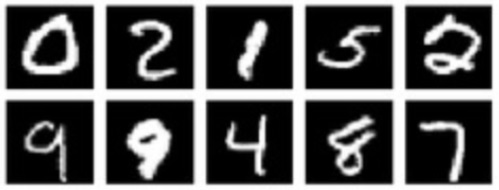
\includegraphics[scale=1]{mnist.png}
  	\caption{Tio bilder av handskrivna siffror från MNISTdatabasen. \cite{MNIST}}
\end{figure}

Input för modellen är en $R \times 1 \times 28 \times 28$ tensor där R står för mini-hopstorleken. Modellen prognostiserar tio värden per bild i form av en tensor $\hat{y} \in \mathbb{R}^{R \times C}$, ett värde för varje klass $C=10$ av siffra. Konstandsfunktionen som har minimerats under träningstiden är funktionen \textit{cross-entropy} betecknat med L. Den verkar på två sannolikhetsfördelningar: De verkliga sannolikheterna $y$ och de prognostiserade sannolikheterna $\hat{y}$: \cite{cs231n} \cite{notesonbackprop}
\begin{equation}
L(W) = - \sum^{R-1}_{r=0} \sum^{C-1}_{c=0}y_{r,c} \ \log{\hat{y}_{r,c}}
\end{equation}
\begin{equation}
\pd{L(W)}{\hat{y}_{r',c'}} = - \frac{y_{r',c'}}{\hat{y}_{r',c'}}
\end{equation}
Endast en modell tränades på grund av begränsningar i datakraft. Den bestod av tre stycken konvolutionsblock, följt med ett softmaxlager (se figur 10). En mini-hopstorlek av 50 användes och 5000 iterationer av framåt- och bakåtpropagering kördes på min egenimplementerade modell skriven i python. Totalt tog det 4 timmar att träna nätverket på min CPU. 

Den slutgiltiga precisionen blev $99.2\%$ på 10 000 nya handskrivna siffror modellen aldrig hade sett tidigare. Av 10 000 handskrivna siffror lyckades modellen klassifisera 9 919 siffror rätt.

\begin{figure}[h]\label{MNISTmodel}
	\centering
  		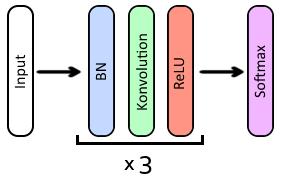
\includegraphics[scale=1.2]{MNISTmodel.png}
  	\caption{Modellen som användes för att läsa av handskrivna siffror. Batch Normalization benämns med BN, konvolution menas en konvolution med kärnstorlek k = 5 och stride s = 2. ReLU är aktiveringsfunktionen Rectified Linear Units och softmax är softmaxlagret.}
\end{figure}

\subsubsection{Dense Face Detection and Localization}
Ett konvolutionellt neuralt nätverk är anpassat för att detektera upp till flera tusen ansikten åt gången för realtidsvideo. Modellen producerar ett bestämt antal \textit{boudning boxes}: koordinater som ska detektera alla olika objekt i bilden. Jag utgick från architekturen från RetinaNet från \textit{Focal Loss for Dense Object Detection} (Lin et al.) och anpassade den till $K = 1$ klasser. I varje position i outputlagret föreslår modellen en \textit{boudning box} med fyra koordinater: två punkter för det övre vänstra hörnet respektive nedre hörna hörnet av den positionens \textit{bounding box}. Utöver det förutsägs det $K+1$ sannolikheter att \textit{bounding boxen} innehåller ett objekt av alla $K$ förgrundklasser och 1 bakgrundklass (lådan innehåller inga objekt).\cite{cs231n}\cite{retinanet}

Modellen för objektdetektering går ut på att man utgår från ett antal så kallade anchor boxes vid varje rumslig position i det sista konvolutionella lagret. Om lagret har bredden och höjden $W$ respektive $H$ och $A$ olika storlekar på anchor boxes har lagret totalt $WHA$ olika anchor boxes. Vid träning tilldelas en anchor box ett objekt om dens \textit{intersection over union} (IoU) med den verkliga bounding boxen är större än 0.5 (se figur 11 IoU används för att beräkna hur lika två olika mängder är. I detta fall är mängderna areorna av en anchor box och ett objekts verkliga bounding box. IoU definieras som storleken av snittet av två mänger $A$ och $B$ dividerat med storleken av unionen av $A$ och $B$: \cite{cs231n} \cite{iou}

\begin{equation}
IoU(A, B)=\frac{|A \cap B|}{|A \cup B|}
\end{equation}

\begin{figure}[h]\label{figiou}
	\centering
  		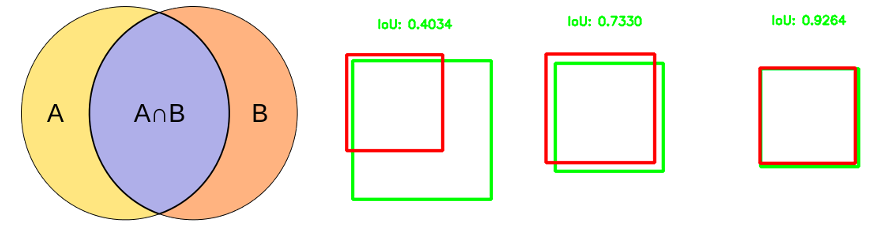
\includegraphics[scale=0.5]{iou.png}
  	\caption{IoU definieras som storleken av snittet av två mänger A och B dividerat med storleken av unionen av A och B. En större IoU medför att prognosen är närmare sanningen. \cite{iou}}
\end{figure}

RetinaNet använder sig av en \textit{feature pyramid}-arkitektur beskriven i \textit{"Feature Pyramid Networks for Object Detection"} (Lin et al.) och en ResNet101 (He et al.) som \textit{backbone}. Featurepyramiden används för att få ut \textit{feature maps} från olika delar av det konvolutionella neurala nätverket för att kunna detektera objekt av olika storlekar. Varje pyramidnivå matas in i ett klassifikationshuvud respektive regressionshuvud (se figur 12) för att räkna ut sannolikheterna att varje anchor box innehåller de $K+1$ olika klasserna, samt att förfina varje anchor box koordinater genom att prognostisera 4 olika offsets för varje sida av anchor boxens bounding box. \cite{resnet} \cite{retinanet} \cite{fpn} 

\begin{figure}[h]\label{figiou}
	\centering
  		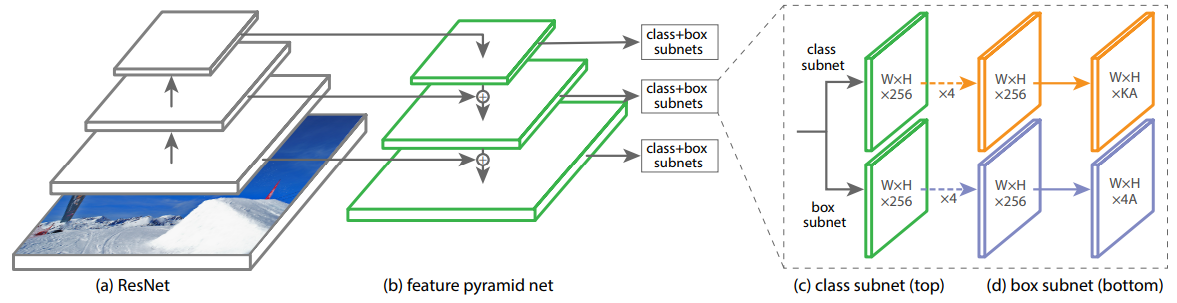
\includegraphics[scale=0.38]{retinanet.png}
  	\caption{RetinaNets arkitektur från \textit{Focal Loss for Dense Object Detection} (Lin et al.). Varje pyramidnivå matas in i ett klassifikationshuvud och ett regressionshuvud. \cite{retinanet}}
\end{figure}

Till skillnad från RetinaNet har min modell, FaceNet, ett mindre antal pyramidnivåer för att lätta på beräkningskraften och för att detektera mindre objekt. RetinaNets anchors har areor från $32^2$ till $512^2$ pixlar spridda över pyramidnivåer P3 till P7. FaceNet använder sig av areor $14^2$ till $220^2$ pixlar spridda över pyramidnivåer P3 till P6. Regressionshuvudet och klassifikations- huvudet i RetinaNet består av 5 konvolutionslager med kärnstorlek 3. Facenet använder istället 2 och 3 konvolutionslager för regressionshuvudet respektive klassifikationshuvudet. I det originala Feature Pyramidnätverket användes linjär interpolation för att göra storleken av högre feature maps större. I FaceNet används k-nearest neighbors (k-NN) istället. ResNet50 användes istället för ett ResNet101 som backbone för att lätta på beräkningskostnaderna. \cite{resnet} \cite{retinanet} \cite{fpn} 

Kostnadsfunktionen som användes var en kombination av Focal Loss (Lin et al.) och Smooth L1 Loss. FaceNet använder samma hyperparametrar som uppnådde bästa resultat för RetinaNet: $\alpha = 3$ för förgrundklassen och $\gamma=2$. \cite{retinanet}

\begin{equation}
L_r(x) = \begin{cases}
				0.5x^2 & \mbox{om } |x| < 1\\
				|x| - 0.5 & \mbox{i annat fall}\\
			\end{cases}
\end{equation}

\begin{equation}
L_c(p, \hat{p}) = - \alpha (1-p)^{\gamma}p \log{\hat{p}}
\end{equation}

\begin{equation}
\begin{split}
	L(W) = & \sum_{k \in pyramid} \frac{1}{N^k_c} \sum_{a \in anchors} L_r(r_a - \hat{r}_a) \\ 
	& + \sum_{k \in pyramid} \frac{1}{N^r_c} \sum_{a \in anchors} L_c(p_a, \hat{p}_a)  \\ 
\end{split}
\end{equation}

$N^k_c $ och $N^k_r $ betäcknar alla anchors som deltar i klassifikationskonstnaden respektive regressionskonstnaden i pyramidnivå $k$. För klassifikationskonstnaden är $\hat{p}$ 1 för alla anchors som har blivit tillgivna ett objekt och 0 för alla som bara innehåller bakgrundsklassen. Endast anchors som innehåller ett objekt deltar i regressionskostnaden. $r_a$ innehåller de 4 koordinaterna den slutgiltiga boudning boxen har.

Modellen tränades i 350 000 iterationer med en mini-hopsstorlek av 3. Träningshastigheten började på 0.005 och dividerades med 10 vid 200 000 iterationer. Varje träningsexempels storlek gjordes slumpmässigt om till $512^2$, $576^2$ eller $640^2$ pixlar och speglades horizontellt med sannolikhet 0,5 för att artificiellt utöka mängden träningsdata. Den totala träningstiden var 18 timmar på en NVIDIA GTX 1080ti. Figur 13 visar kvantitativa resultat från WIDERFace valideringsdata.

En iteration av framåtpropageringen tar 20 ms vilket möjliggör att modellen kan köras i realtid, 50 gånger i sekunden.

\begin{figure}[h]\label{results1}
	\centering
  		
\includegraphics[scale=0.42]{results1.png}
  	\caption{Kvantitativa resultat från valideringsdatan från WIDERFace: Bilder som modellen aldrig har sett tidigare.}
\end{figure}

\section{Diskussion}
Vad är ett konvolutionellt neuralt nätverk?
Hur härleds framåt- och bakåtpropagering i konvolutionella neurala nätverk?
Hur kan modellen tillämpas för att implementera sifferavläsning, ansiktsigenkänning och objektdetektering i bilder?

Den matematiska modellen av artificiella neurala nätverk och konvolutionella neurala nätverk, samt bakåt- och framåtpropagering förklaras och härleds i sektion 3.2 och 3.3. Ett exempel på hur modellen kan tillämpas är att klassificera handskrivna siffror, som i sektion 3.4.1. 
En annan möjlighet är att anpassa ett konvolutionellt neuralt nätverk för att detektera alla ansikten i en digital bild. På grund av att en iteration av algoritmen tar 20 ms är det möjligt att köra modellen i realtid. Det kan exempelvis användas i övervakningskameror eller inom robotik för att känna igen människoansikten i realtid. 

Algoritmen är dock inte perfekt och har flera brister. Modellen prognostiserar att det finns ansikten på flera ställen där det inte finns några i verkligheten. För att undankomma detta låter jag endast modellen visa upp bounding boxes med sannolikhet större än 0.5 att det finns ett ansikte där. Resultatet blir att modellen inte hittar 100\% av all ansikten i bilden (se figur 13). Ytterligare har modellen problem med små ansikten. Detta är dels på grund av att modellen inte kan urskilja ett ansikte med så lite information (ca minimum $10^2$ pixlar per ansikte), och dels för att FaceNet prognostiserar ca 30 000 olika anchors för de minsta storlekarna. Detta leder till att klassifikationskostnaden består av till mestadels negativa exempel. Delta-felet av bakgrundsklasserna dominerar och gör att delta-felet av förgrundsklassen (ansikten) inte har en stor påverkan på den slutgiltiga gradienten.


\begin{thebibliography}{99}	
\bibitem{cs231n} 
	\textit{CS231n: Convolutional Neural Networks for Visual Recognition.}
    F. Li, A. Karpathy och J. Johnson.
	Stanford University, föreläsning, vinter 2016.
	
\bibitem{wikiStanford} 
	\textit{Unsupervised Feature Learning and Deep Learning.}
    Standford University, Department of Computer Science.
    URL http://ufldl.stanford.edu/wiki/.
	Senast uppdaterad 31 mars 2013.	
	
\bibitem{notesonbackprop} 
	\textit{Notes on Backpropagation.}
    P. Sadowski.
    University of California Irvine	Department of Computer Science.
    
\bibitem{convmath} 
	\textit{Introduction to Convolutional Neural Networks.}
    J. Wu. 
    National Key Lab for Novel Software Technology, Nanjing University, Kina.
    1 maj, 2017.

\bibitem{convarithmetic} 
	\textit{A guide to convolution arithmetic for deep learning.}
    V. Dumoulin  och F. Visin.
    FMILA, Université de Montréal. AIRLab, Politecnico di Milano.
	24 mars, 2016.

\bibitem{highperformanceconv} 
	\textit{High Performance Convolutional Neural Networks for Document Processing.}
    K. Chellapilla, S. Puri, P. Simard.
    Tenth International Workshop on Frontiers in Handwriting Recognition. 
    La Baule, Frankrike, Suvisoft.
	Oktober 2006.


	
\bibitem{gradient} 
	\textit{Scientific Computing 2013, Worksheet 6: Optimization: Gradient and steepest descent.}
    University of Tartu, Estland.
    2013.
    
\bibitem{yolo} 
	\textit{You only look once: Unified, real-time object detection.}
    J. Redmon, S. Divvala, R. Girshick, och A. Farhadi. 
    arXiv preprint arXiv:1506.02640, 2015.
    
\bibitem{batchnorm} 
	\textit{Batch normalization: Accelerating deep network training by reducing internal covariate shift.}
    S. Ioffe och C. Szegedy. 
	arXiv preprint arXiv:1502.03167, 2015.
    
\bibitem{webconv1} 
	\textit{Backpropagation In Convolutional Neural Networks.}
	J. Kafunah.
    DeepGrid, Organic Deep Learning. 
    URL http://www.jefkine.com/.
	5 september 2016.

\bibitem{webBN1} 
	\textit{What does the gradient flowing through batch normalization looks like?}
	C. Thorey.
    Machine Learning Blog. 
    URL http://cthorey.github.io/.
	28 januari 2016.
	
\bibitem{webconv2} 
	\textit{Note on the implementation of a convolutional neural networks.}
	C. Thorey.
    Machine Learning Blog. 
    URL http://cthorey.github.io/.
	2 februari 2016.
	
\bibitem{webBN2} 
	\textit{Understanding the backward pass through Batch Normalization Layer.}
	Flaire of Machine Learning
    URL https://kratzert.github.io.
	5 september 2016.
	
\bibitem{webconv3} 
	\textit{Convolutional Neural Networks.}
	A. Gibiansky.
    URL http://andrew.gibiansky.com.
	24 februari 2014.
	
\bibitem{websoftmax} 
	\textit{Classification and Loss Evaluation - Softmax and Cross Entropy Loss.}
	P. Dahal. 
	DeepNotes.
    URL https://deepnotes.io/softmax-crossentropy.
	24 februari 2014.
	
\bibitem{MNIST}
	\textit{The MNIST database of handwritten digits}
	Y. LeCun, C. Cortes och C. Burges. Courant Institute, NYU. Google Labs, New York. Microsoft Research, Redmond. 
	URL http://yann.lecun.com/exdb/mnist/.
	Hämtad 3 november 2017.
	
\bibitem{figSGD}
	\textit{Pygradsc.}
	J. Komoroske.
	URL https://github.com/joshdk/pygradesc.
	12 oktober 2012.
	
\bibitem{figboatcnn}
	\textit{Understanding Convolutional Neural Networks for NLP.}
	D. Britz.
	WildML, Artificial Intelligence, Deep Learning, and NLP.
	7 november 2015.
	
\bibitem{figkonv}
	\textit{Understanding Convolutional Neural Networks for NLP.}
	D. Britz.
	WildML, Artificial Intelligence, Deep Learning, and NLP.
	7 november 2015.
	
\bibitem{figconv}
	\textit{Deep learning for complete beginners: convolutional neural networks with keras.}
	P. Veličković.
	Camebridge Spark. 
	URL https://cambridgespark.com/content.
	Senast uppdaterad 20 mars 2017.


\bibitem{resnet} 
	\textit{Deep residual learning for image recognition.}
    K. He, X. Zhang, S. Ren, och J. Sun. 
    arXiv preprint arXiv:1512.03385, 2015.

\bibitem{iou}
	Jaccard Index. Wikipedia.
    URL https://en.wikipedia.org/wiki/Jaccard{\_}index. 
    Hämtad 20 januari 2018
    
\bibitem{retinanet}
	\textit{Focal Loss for Dense Object Detection.}
	Tsung{-}Yi Lin,
    Priya Goyal,
    Ross B. Girshick,
    Kaiming He and
    Piotr Doll{\'{a}}r.
    arXiv preprint arXiv:1708.02002, 2017

\bibitem{fpn}
	\textit{Feature Pyramid Networks for Object Detection.}
	Tsung{-}Yi Lin,
               Piotr Doll{\'{a}}r,
               Ross B. Girshick,
               Kaiming He,
               Bharath Hariharan and
               Serge J. Belongie.
    arXiv preprint arXiv:1612.03144, 2016
    
\bibitem{WIDERFace}
	\textit{WIDER FACE: A Face Detection Benchmark.}
	Yang, Shuo and Luo, Ping and Loy, Chen Change and Tang, Xiaoou
    IEEE Conference on Computer Vision and Pattern Recognition (CVPR), 2016

\end{thebibliography}


\end{document}